\documentclass[a0paper, portrait]{tikzposter}
\usepackage[utf8]{inputenc}
\usepackage{authblk}
\makeatletter
\renewcommand\maketitle{\AB@maketitle} % revert \maketitle to its old definition
\renewcommand\AB@affilsepx{\quad\protect\Affilfont} % put affiliations into one line
\makeatother
\renewcommand\Affilfont{\Large} % set font for affiliations
\usepackage{adjustbox}
\usepackage[labelformat=empty]{caption}

%%%%%%%%%%%%%%%%%%%%%%%%
%  table env for tkiz  %
%%%%%%%%%%%%%%%%%%%%%%%%
\newcounter{tablecounter}
\newenvironment{tikztable}[1][]{
  \def \rememberparameter{#1}
  \vspace{10pt}
  \refstepcounter{tablecounter}
  \begin{center}
  }{
    \ifx\rememberparameter\@empty
    \else
    \\[10pt]
    {\small \rememberparameter}
    \fi
  \end{center}
}
\renewenvironment{tikzfigure}[1][]{
  \def \rememberparameter{#1}
  \vspace{10pt}
  \refstepcounter{figurecounter}
  \begin{center}
  }{
    \ifx\rememberparameter\@empty
    \else %nothing
    \\[10pt]
    %{\small Fig.~\thefigurecounter: \rememberparameter}
    {\small \rememberparameter}
    \fi
  \end{center}
}
%%%%%%%%%%%%%%%%%%%%%%
 
\title{\parbox{\linewidth}{\centering The Genetic Architecture of Human Aggression}}

\author[1,2]{Robert M. Porsch}
\author[4]{Meike Bartels}
\author[4]{Dorret Boomsma}
\author[1,2,4]{Pak C. Sham}
\author[1,2,4]{Stacey S. Cherny}
\affil[1]{State Key Laboratory of Brain and Cognitive Sciences, University of Hong Kong}
\affil[2]{Department of Psychiatry, University of Hong Kong}
\affil[3]{Department of Biological Psychology, VU University Amsterdam}
\affil[4]{Center of Genomic Science, University of Hong Kong}
 
\usetheme{Simple}
\usetitlestyle{Filled}
 
\begin{document}

\maketitle
 
\begin{columns}
  \column{0.5}
  \block{Introduction}{ 
    \begin{itemize}
      \item Aggression has beneficial and harmful consequences 
      \item A highly heritable trait
      \item Potential sex differences in the genetic architecture are unclear
      \item Specific genetic loci remain unidentified
      \item Unknown genetic overlap with related phenotypes
    \end{itemize}
  }

  % Methods and Samples
  \block{Description of Samples}{
    \textbf{Twin Data:}\\
        \begin{tikztable}[Overview of twin data]
          \input{tables/twins.tex}
        \end{tikztable}
    \adjustbox{valign=t}{
      \begin{minipage}{0.29\linewidth}
        \textbf{The UK BioBank}\\
        \begin{itemize}
          \item 40--69 years old
          \item Aggression was measured on a single yes/no item
          \item All subjects were genotyped
        \end{itemize}
      \end{minipage}
    }
    \adjustbox{valign=t}{
      \begin{minipage}{0.79\linewidth}
        \vspace{2cm}
        \begin{tikztable}[Sample Size and Missingness of UK Biobank]
          \input{tables/descriptive_ukb.tex}
        \end{tikztable}
      \end{minipage}
    }
  }

  \block{Twin Modeling Results}{
    \begin{itemize}
      \item Heritability ranges between 42\%-78\% (female) and 59\%-68\% (male)
      \item High Stability of Genetic Factors: \\
        Genetic Correlation NTR:\@ $0.76-0.85$ \\
        Genetic Correlation TEDS:\@ $0.64-0.77$ 
      \item Small but significant quantitative sex differences
      \item Genetic factors are the major source of stability
      \item Shared environmental influence are present, especially in boys
    \end{itemize}
  }
  % Association Results
  \block{Phenotypic Effects}{

    \begin{minipage}{0.49\linewidth}
      \begin{tikzfigure}[Phenotypic Correlations]
        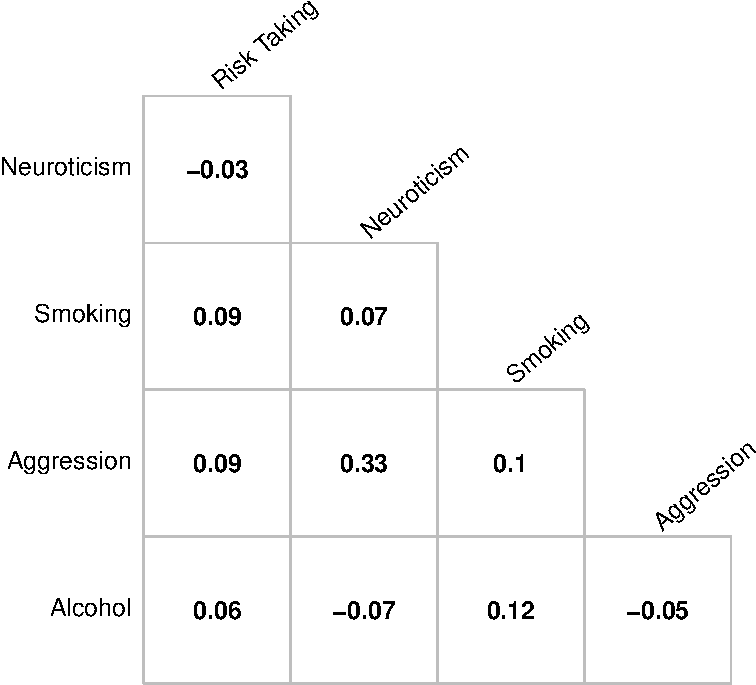
\includegraphics[width=0.8\linewidth]{../ukb_assoc/figure/phenotype/corr_plot_ci.pdf}
      \end{tikzfigure}
    \end{minipage} \hfill
    \begin{minipage}{0.49\linewidth}
      \begin{tikzfigure}[
        Effects of Age and Sex (male=1, female=0)]
        \includegraphics[width=0.99\linewidth]{descriptive_plots_poster.pdf}
      \end{tikzfigure}
    \end{minipage}
  }
  % Genetic Correlation Matrix
  \block{Genome Wide Association Study}{
    %\begin{minipage}{0.49\linewidth}
    %  \begin{tikzfigure}[QQ-Plot of aggression GWAS]
    %    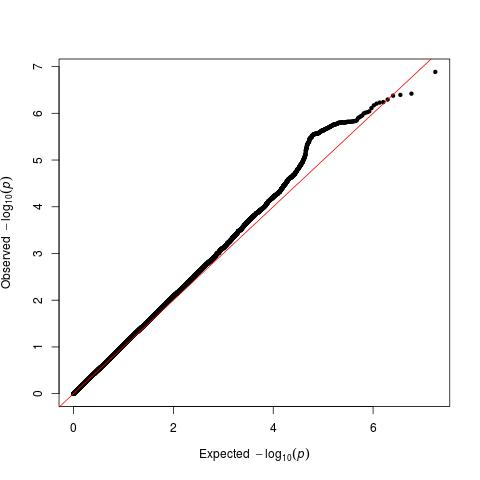
\includegraphics[width=0.99\linewidth]{{../ukb_assoc/figure/qq_plots/qq_plot_4526}.jpeg}
    %  \end{tikzfigure}
    %\end{minipage}
    %\begin{minipage}{0.49\linewidth}
    %\end{minipage}
    \begin{itemize}
      \item No Genome-wide significant signal was identified
      \item Improved sample size or better phenotyping required
    \end{itemize}
    \begin{tikzfigure}[Manhattan plot of aggression GWAS]
      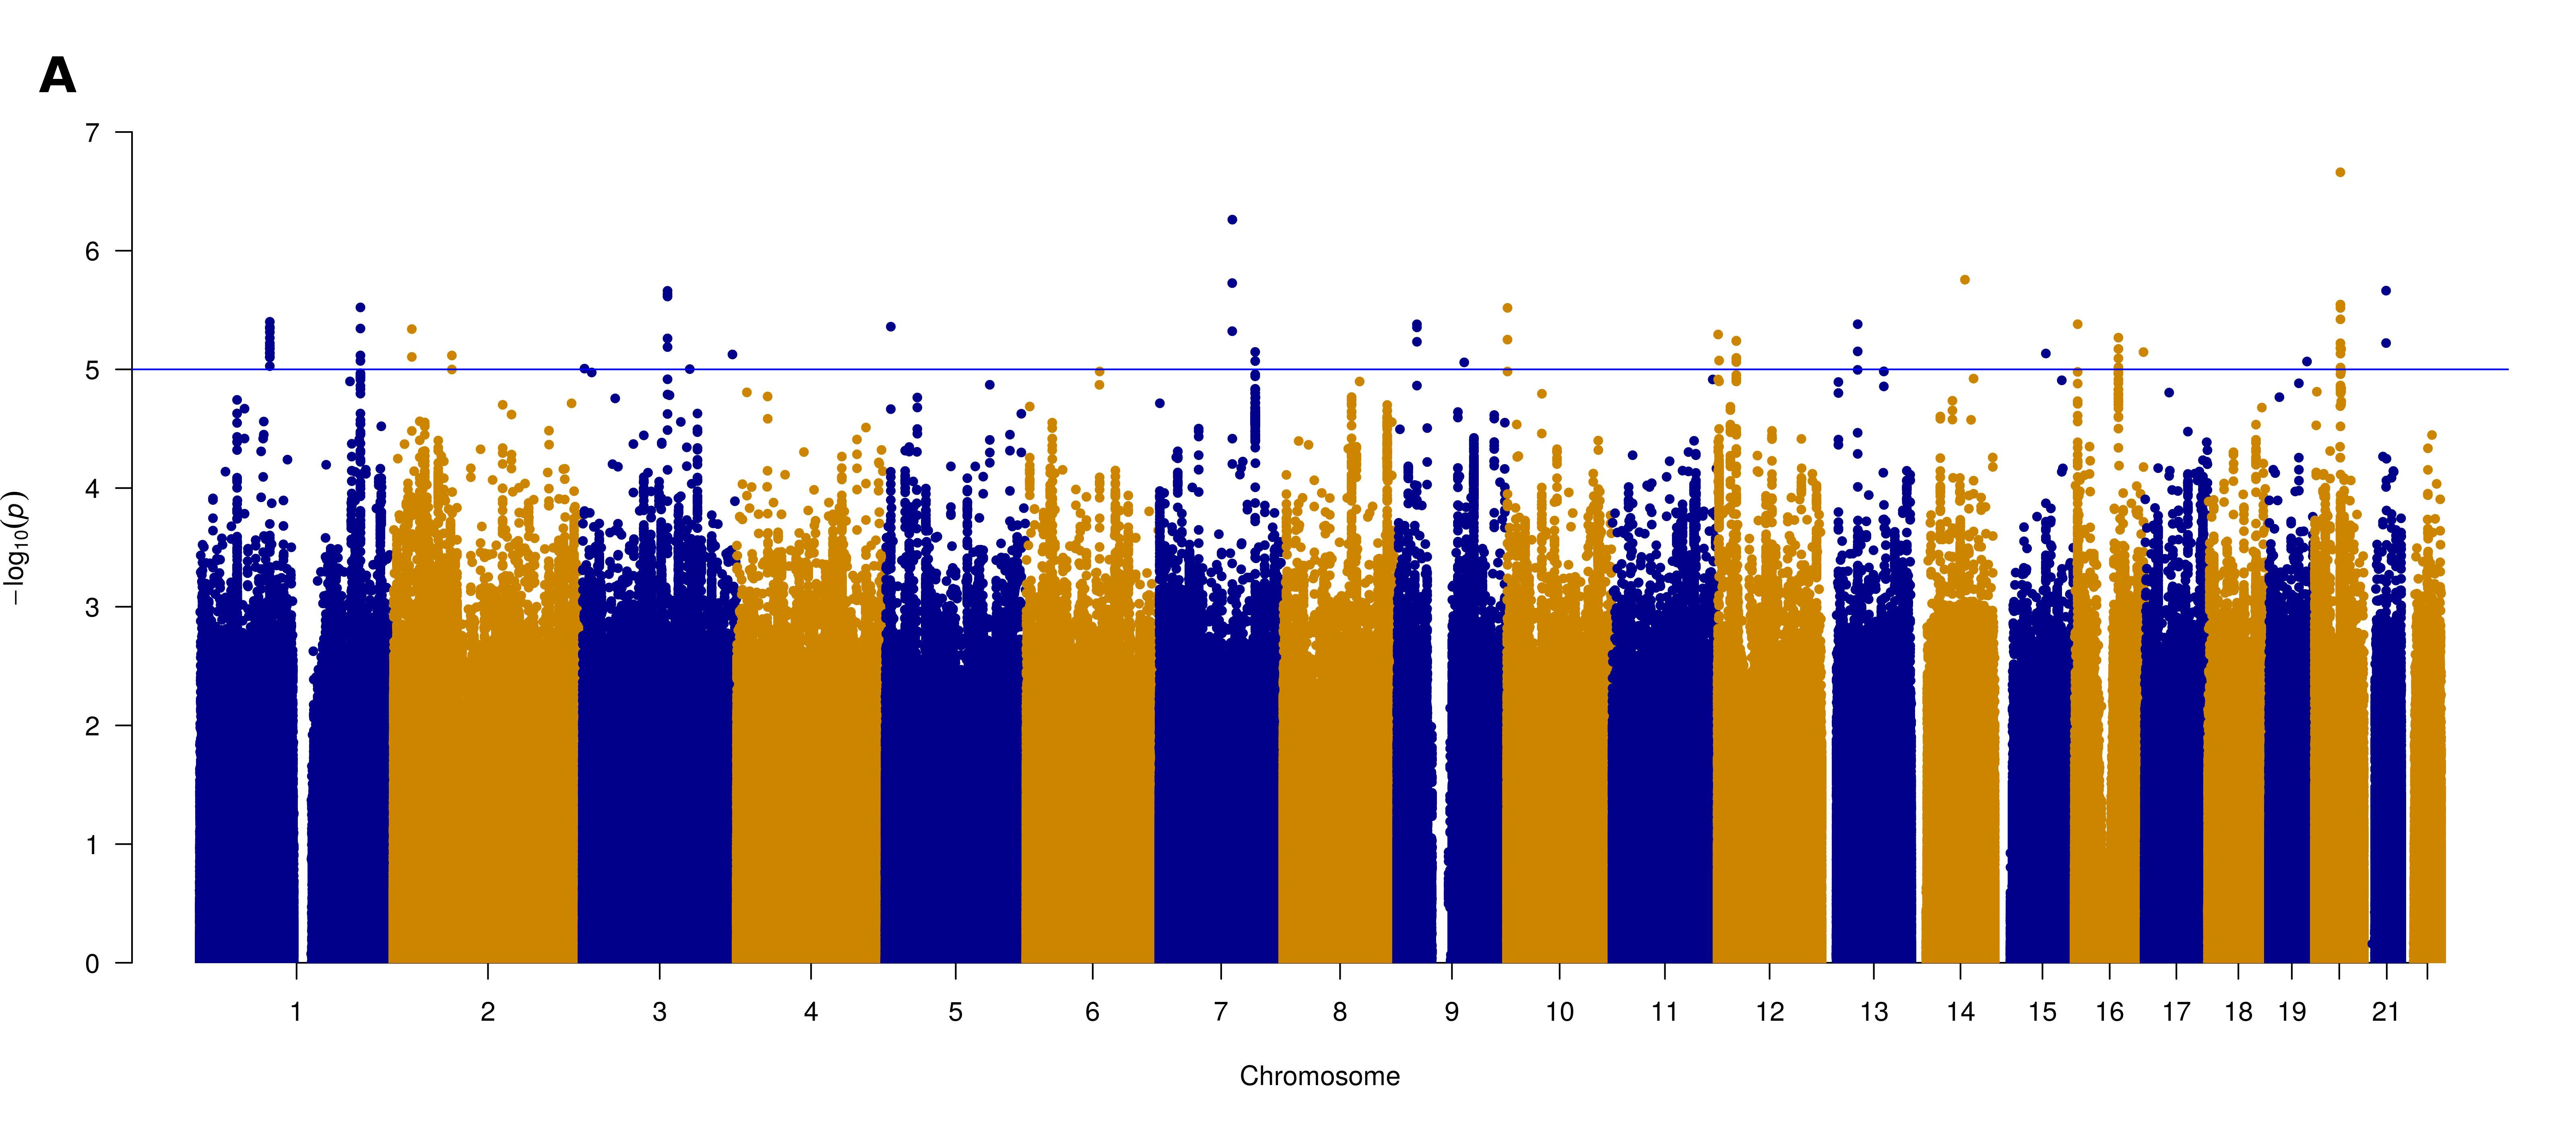
\includegraphics[width=0.7\linewidth]{../ukb_assoc/figure/manhatten_plots/agg_manhatten_color_2_A.jpeg}
    \end{tikzfigure}
  }


  \column{0.5}


  \block{Genetic Correlations}{
    \begin{tikzfigure}[Genetic Correlations within the UKB]
      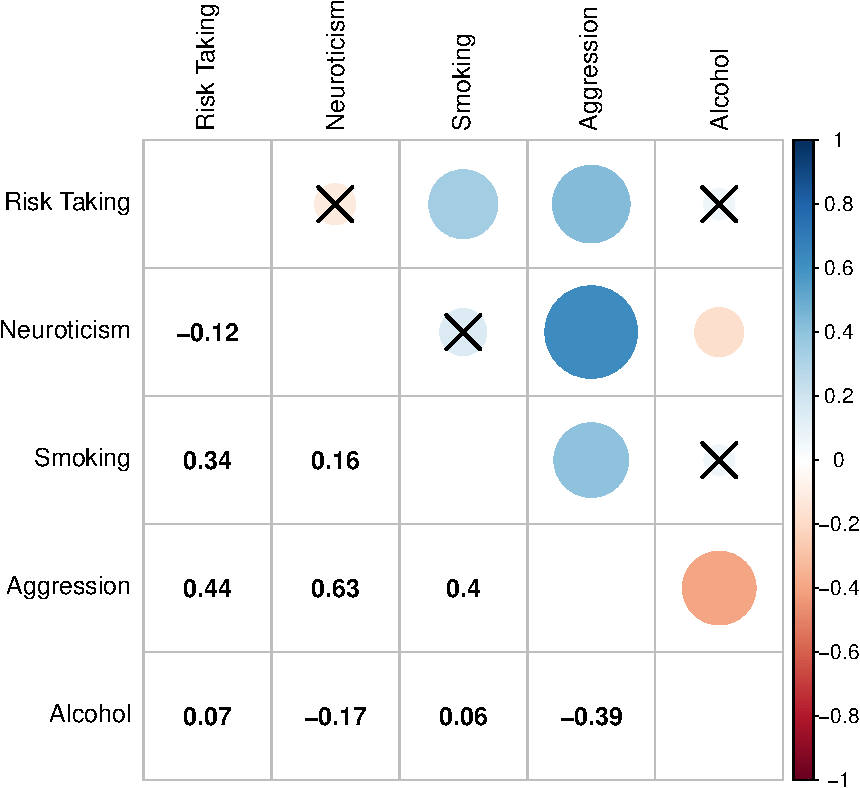
\includegraphics[width=0.65\linewidth]{../ukb_assoc/figure/genetic_corr/gcorr_plot_circle_full_se.pdf}
    \end{tikzfigure}
  }

  % Phenotypic Effects

  % MR
  \block{Estimating Causality: Mendelian Randomization}{
    \textbf{What is Mendelian Randomization (MR)?}
    \begin{itemize}
      \item Infers potential causal effects from observational data 
      \item Natural randomized control trial
      \item Estimating the causal effects of Schizophrenia (SZ), Major Depressive Disorder (MDD), Depressive Symptom (DS) and Bipolar Disorder (BP) on aggression and risk taking
    \end{itemize}

    \begin{tikzfigure}[
      Estimated causal effect of psychiatric disorders on impulsive aggression (A) and risk taking (B).
      ]\label{fig:overall_mr_effect}
      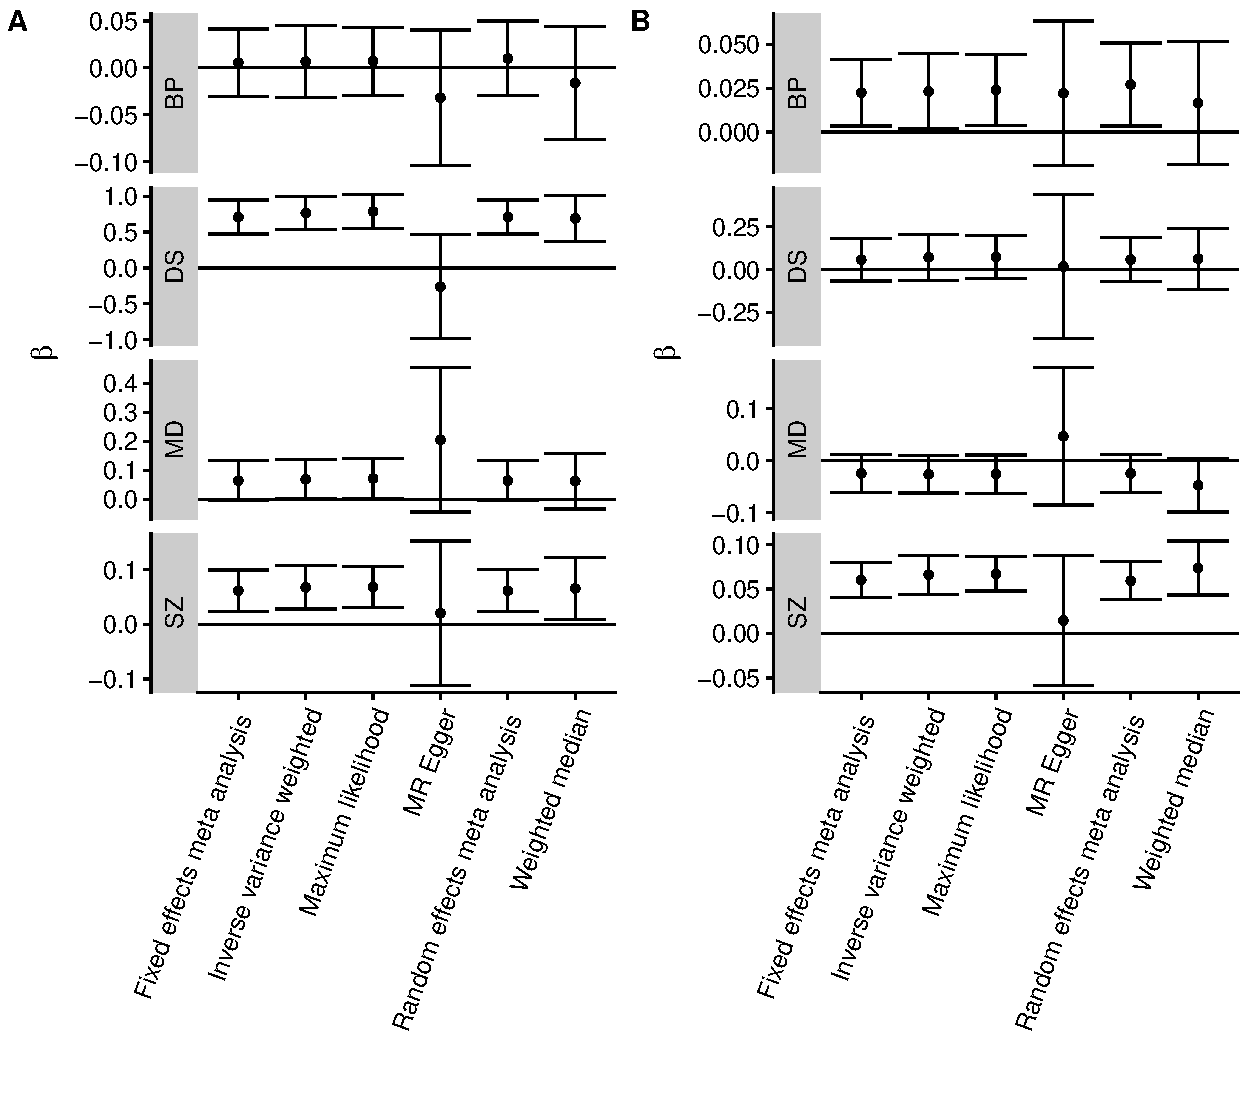
\includegraphics[width=0.8\linewidth]{../ukb_psychiatric/figures/overall_mr_effect.pdf}
    \end{tikzfigure}

    \textbf{Results of MR:}
    \begin{itemize}
      \item Estimated causal effects are small
      \item Some indication for a causal connection between SZ and aggression/risk taking
    \end{itemize}
  }

  \block{Conclusion}{
    \begin{itemize}
      \item Heritability: Twin Studies (42\% to 78\%), GWAS (5\%)
      \item Small quantitative sex differences in genetic factors
      \item Limited sample size for aggression GWAS
      \item Suggested causal connection between schizophrenia and aggression \& risk taking
      \item Independent replication of findings needed
    \end{itemize}

    \textbf{Acknowledgment:}\\
    HKSAR - Innovation and Technology Commision -- TIC Fund (ITF)
  }

\end{columns}

\end{document}
